\documentclass[12pt,a4paper]{article}

\usepackage[utf8]{inputenc}
\usepackage[T1]{fontenc}
\usepackage[brazil]{babel}
\usepackage{amsmath}
\usepackage{booktabs}
\usepackage{geometry}
\usepackage{array}
\usepackage{float}
\usepackage{graphicx}

\geometry{
    left=3cm,
    right=2cm,
    top=3cm,
    bottom=2cm
}

\renewcommand{\thesection}{\arabic{section}.}
\renewcommand{\thesubsection}{\arabic{section}.\arabic{subsection}.}

\title{\textbf{Questão 4.1 -- Análise da Série Temporal de \texttt{total\_user}\\
Sistema de Compartilhamento de Bicicletas}}
\author{}
\date{}

\begin{document}

\maketitle

\section{Introdução}

O primeiro item da Questão 4 tem como objetivo analisar o comportamento temporal
da utilização do sistema de compartilhamento de bicicletas por meio da variável
\texttt{total\_user}. Para isso, foi construída uma série temporal considerando
as observações diárias do conjunto de dados específico do grupo, formado por 300
registros consecutivos.

A variável \texttt{total\_user} representa o número total de usuários do sistema
em cada dia e é obtida pela soma entre o número de usuários casuais e registrados:

\begin{equation}
\text{total\_user}_i =
\text{casual}_i + \text{registered}_i,
\end{equation}

em que $i$ representa cada observação diária.

A análise da série temporal permite identificar períodos de maior e menor
utilização do sistema, além de observar tendências e oscilações ao longo do
período analisado.

\section{Construção da série temporal}

Para a construção da série temporal, as observações foram organizadas em ordem
cronológica utilizando a variável \texttt{dteday}. No eixo horizontal do gráfico
foram representadas as datas das observações, enquanto no eixo vertical foi
representado o número total de usuários em cada dia.

A Figura \ref{fig:serie-temporal} apresenta a evolução diária da variável
\texttt{total\_user} durante o período analisado.

\begin{figure}[H]
    \centering
    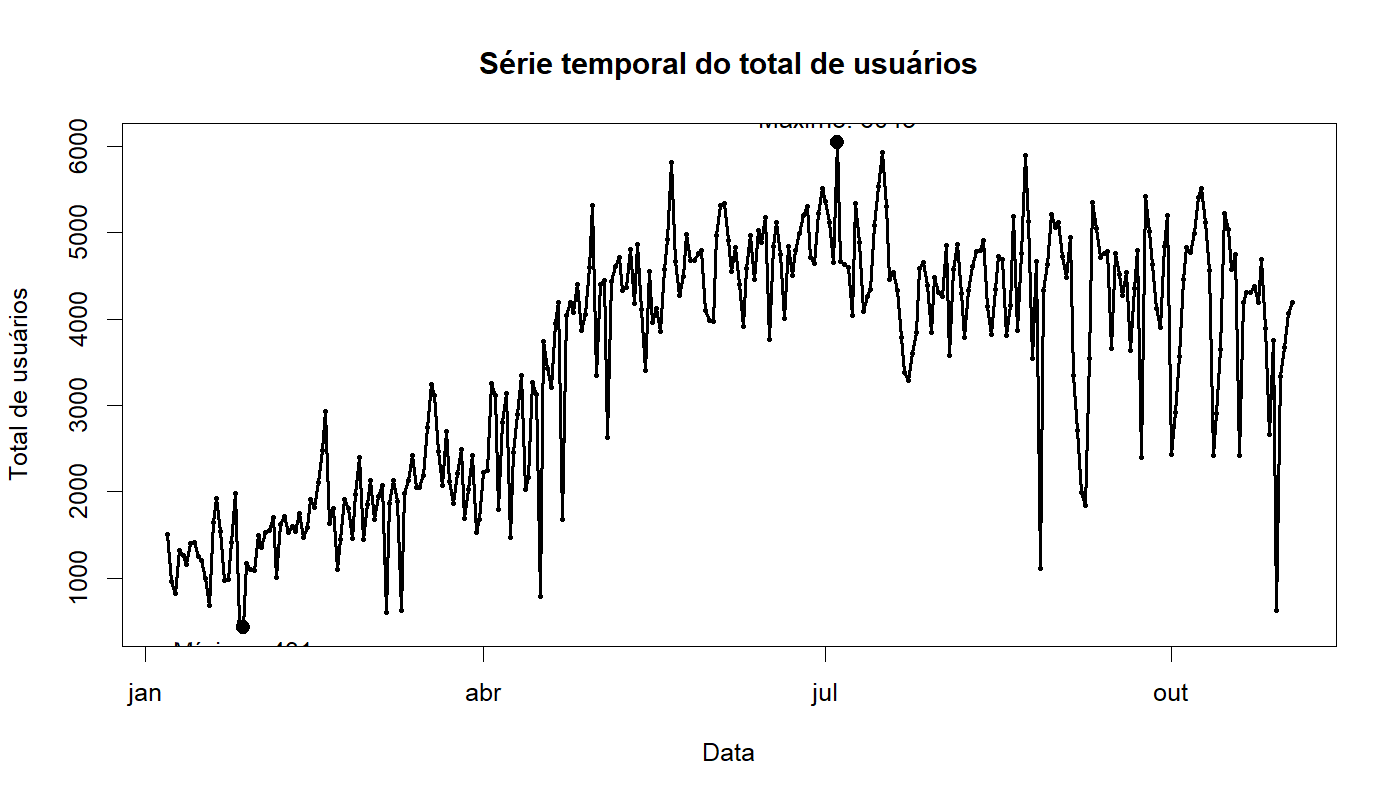
\includegraphics[width=0.95\textwidth]{4.1.serie_temporal_total_user.png}
        \caption{Série temporal do número total de usuários do sistema.}
    \label{fig:serie-temporal}
\end{figure}

A representação gráfica evidencia variações diárias importantes na utilização
do sistema, além de mudanças no nível geral de demanda ao longo dos meses.

\section{Identificação dos valores máximo e mínimo}

A partir da série temporal, foram identificadas as observações correspondentes à
maior e à menor utilização do sistema no conjunto analisado.

\begin{table}[H]
\centering
\caption{Maior e menor utilização observadas no período}
\begin{tabular}{lcc}
\toprule
\textbf{Situação} & \textbf{Data} & \textbf{Total de usuários} \\
\midrule
Maior utilização & 04/07/2011 & 6043 \\
Menor utilização & 27/01/2011 & 431 \\
\bottomrule
\end{tabular}
\end{table}

O maior valor registrado ocorreu em 04 de julho de 2011, quando foram
contabilizados 6043 usuários. Em contraste, o menor valor do período foi
observado em 27 de janeiro de 2011, com 431 usuários.

\section{Análise dos períodos de maior e menor utilização}

\subsection{Período de menor utilização}

Nos primeiros meses da série, especialmente durante janeiro e fevereiro,
observam-se níveis de utilização relativamente menores. Grande parte das
observações desse período encontra-se em patamares inferiores aos verificados
nos meses posteriores.

O menor valor de toda a série ocorre em 27 de janeiro, com 431 usuários. Além
desse ponto mínimo, o início da série apresenta diversos dias com valores
próximos ou inferiores a aproximadamente 2000 usuários, indicando um período de
demanda reduzida em comparação com os meses seguintes.

\subsection{Período de crescimento da utilização}

Entre março e abril, a série apresenta uma elevação gradual no número total de
usuários. Os valores passam progressivamente de níveis próximos de 2000 usuários
para observações frequentemente superiores a 3000 e 4000 usuários.

Esse comportamento caracteriza uma mudança importante no nível de utilização do
sistema. Embora permaneçam algumas quedas pontuais, o comportamento geral indica
aumento da demanda ao longo desse intervalo.

\subsection{Período de maior utilização}

A partir de maio, a série passa a apresentar valores predominantemente mais
elevados. Entre maio e julho, grande parte das observações encontra-se entre
aproximadamente 4000 e 5500 usuários.

O ponto máximo da série ocorre em 04 de julho de 2011, com 6043 usuários. Esse
resultado está inserido em um período no qual vários dias também apresentam
valores próximos ou superiores a 5000 usuários, caracterizando uma fase de
utilização elevada do sistema.

\subsection{Comportamento após o valor máximo}

Após julho, o número total de usuários permanece elevado em muitos dias, porém
a série passa a apresentar oscilações mais intensas.

Entre agosto e outubro, são observados diversos valores entre aproximadamente
4000 e 5000 usuários, intercalados com quedas acentuadas. Dessa forma, embora o
nível geral de utilização permaneça elevado, a variabilidade diária torna-se
mais evidente.

\section{Principais padrões observados}

A análise da série temporal permite identificar três características principais.
Primeiramente, observa-se uma tendência de crescimento da utilização durante a
primeira metade do período analisado. Os valores registrados em janeiro e
fevereiro são, em geral, inferiores aos observados nos meses seguintes, enquanto
março e abril representam uma fase de transição para níveis mais elevados de
demanda.

Em segundo lugar, entre maio e julho ocorre o período de utilização mais intensa.
Nesse intervalo, os valores permanecem frequentemente acima de 4000 usuários,
culminando no máximo de 6043 usuários em 04 de julho.

Por fim, após o período de crescimento, a série apresenta um nível elevado de
utilização acompanhado de maior variabilidade. Entre agosto e outubro são
observadas sucessivas oscilações, com dias de utilização elevada intercalados
com quedas acentuadas.

\section{Conclusão}

A construção da série temporal de \texttt{total\_user} permitiu visualizar a
evolução da utilização do sistema de compartilhamento de bicicletas ao longo das
300 observações do grupo.

O menor valor observado foi de 431 usuários em 27 de janeiro de 2011, enquanto
o maior valor foi de 6043 usuários em 04 de julho de 2011. A série apresenta
níveis relativamente baixos no início do período, seguidos por crescimento
progressivo durante março e abril.

Entre maio e julho, a utilização atinge seus maiores níveis, com grande
concentração de observações acima de 4000 usuários. Após esse período, a demanda
permanece relativamente elevada, porém acompanhada por oscilações diárias mais
acentuadas.

Dessa forma, a análise temporal evidencia tanto uma tendência de crescimento na
primeira metade do período quanto uma maior variabilidade na segunda metade,
fornecendo uma visão geral da evolução da demanda pelo sistema ao longo do tempo.

\end{document}